\documentclass{article}

\usepackage{algorithmic, amsmath, amsthm, amsfonts, amssymb,commath, enumerate, tikz, tikz-cd, color, mathrsfs, blindtext}%tikz is for drawing lattices %tikz-cd is for commutative diagrams
															%color is for making notes in red 
															%mathrsfs is for power set font
%\usepackage[mathscr]{eucal} %mathscr gives nice script fonts

\newtheoremstyle{problemstyle}  % <name> This is my problemstyle. use begin{problem}.
        {12pt}                                               % <space above>
        {}                                               % <space below>
        {}                               % <body font>
        {}                                                  % <indent amount}
        {\bfseries}                 % <theorem head font>
        {\normalfont\bfseries.}         % <punctuation after theorem head>
        {.5em}                                          % <space after theorem head>
        {}                                                  % <theorem head spec (can be left empty, meaning `normal')>

\theoremstyle{problemstyle}

\newtheorem{problem}{Problem}
\newtheorem{theorem}{Theorem}
\newtheorem{example}{Example}
\newtheorem{detail}{Detail}
\newtheorem{solution}{Solution}
\newtheorem*{proof*}{Proof}
\newtheorem{definition}{Definition}
\newtheorem{proposition}{Proposition}
\newtheorem*{proposition*}{Proposition}

\tikzcdset{every label/.append style = {font = \small}}

\tikzset{%
    symbol/.style={%
        draw=none,
        every to/.append style={%
            edge node={node [sloped, allow upside down, auto=false]{$#1$}}}
    }
}

\title{ \vspace{-10ex} %uncomment to remove vertical space
%title of assignment goes here e.g. "Math 721 Homework 3"
Hartshorne's Algebraic Geometry 
Chapter 1 Notes
}


\author{David L. Meretzky
}


\date{%date assignment is due goes here
November 2nd, 2018
} 


\renewcommand*{\thefootnote}{$\dagger$} %changes default footnote marking to a dagger instead of a number (numbers are sometimes mistaken for citations)

\begin{document}

\maketitle

\subsection*{Affine Varieties}

In these notes, $k$ denotes a fixed algebraically closed field. We let $\mathbb{A}^n_k$ denote affine $n$-space over $k$, that is $\mathbb{A}^n_k = \{(k_1,...,k_n)|k_i \in k\}$. Let $P$ be an element of $\mathbb{A}^n_k$ or just $\mathbb{A}^n$ when the choice of field is clear from context. In particular $P$ is of the form $(k_1,...,k_n)$. Let $A = k[x_1,...,x_n]$, the polynomial ring in $n$ variables over $k$. Elements of $A$ are functions from $\mathbb{A}^n_k$ to $k$. That is, $p(x_1,...,x_n):\mathbb{A}^n_k \rightarrow k$ by $p(P) = p(a_1,...,a_n) \in k$. 

\begin{definition}
Let $f \in A$. Define $Z(f)$ to be the set of zeroes of of $f$, $Z(f) = \{P \in \mathbb{A}^n | f(P) = 0\}$. More generally, if $T \subseteq A$ then define $$Z(T) = \bigcap_{f \in T} Z(f)$$ the intersection of sets of zeroes in $\mathbb{A}^n_k$. 
\end{definition}

\begin{definition}
The ideal generated by a subset of a commutative ring is the intersection of all ideals containing that set. 
\end{definition}

\begin{proposition}
Let $T \subseteq A$. If $\mathfrak{a}$ is the ideal generated by $T$, then $Z(T) = Z(\mathfrak{a})$. 
\end{proposition}

\begin{proof}
Clearly $Z(\mathfrak{a}) \subseteq Z(T)$ because $T \subseteq \mathfrak{a}$. It remains to show the reverse inclusion. 

Suppose $P \in Z(T)$, then for every $f \in T$, $f(P) = 0$. Take any $g \in \mathfrak{a}$, $g$ is of the form $g = g_1f_1 + ... + g_mf_m$ for $g_1,...,g_m \in A$ and $f_1,...f_m \in T$.  Then $g(P) = 0$ and therefore  $Z(T) \subseteq Z(\mathfrak{a})$. 
\end{proof}

\begin{definition}
A ring is notherian if it satisfies the ascending chain condition: For any string of ideals $I_1 \subseteq I_2 \subseteq I_3 \subseteq ...$ there exists an index $n$ such that for all $k > 0$, $I_n = I_{n+k}$. 
\end{definition}

\begin{proposition}
Polynomial rings over algebraically closed fields are notherian. 
\end{proposition}

\begin{proposition}
In a notherian ring any ideal has a finite set of generators. 
\end{proposition}

Here is a definition we will use later. 

\begin{definition}
Let $T \subset of A$. The radical of $T$, denoted $r(T)$, is the set of all $f \in A$ such that for some $q>0$, $f^r \in T$. That is $r(T) = \{f \in A | f^q \in T\}$ for some $q >0$.  
\end{definition}

\begin{definition}
Call $Y \subseteq \mathbb{A}^n$ an algebraic set if there exists a $T \subseteq A$ such that $Y = Z(T)$. Namely, for every $P \in Y$ and for all $f \in T$, we have $f(P) = 0$. 
\end{definition}

\begin{proposition}
The union of two algebraic sets is an algebraic set. The intersection of any family of algebraic sets is an algebraic set. The empty set and the whole space are algebraic sets. 
\end{proposition}

\begin{proof}
Let $Y_1$ be annihilated by $T_1 \subseteq \mathbb{A}^n$ and $Y_2$ be annihilated by $T_2 \subseteq \mathbb{A}^n$. The intersection of $T_1$ and $T_2$ annihilates the union of $Y_1$ and $Y_2$. The intersection of all ideals is the 0 ideal. The annihilator of the whole space is $(0)$.  The union of $T_1$ and $T_2$ annihilates the intersection of $Y_1$ and $Y_2$. The union of all ideals is the entirety of $A$. Thus the empty set is algebraic with annihilator $A$. 
\end{proof}

\begin{definition}
The zarisky topology on $\mathbb{A}^n$ is defined by taking the open sets to be compliments to algebraic sets. The intersection of open sets corresponds by De Morgan's Laws to the union of algebraic sets which thus corresponds to the intersection of ideals. Arbitrary unions of open sets correspond to arbitrary intersection of algebraic sets which correspond to arbitrary unions of ideals. The empty set and the whole space are evidently compliment to one another and are also both algebraic and therefore open.  
\end{definition}

\begin{example}
Consider affine $1$-space, $\mathbb{A}^1 = k$. Every ideal in $A = k[x]$ is principal so every algebraic set is then the zeroes of a single polynomial. Since $k$ is algebraically closed every $f \in k[x]$ factors as $f = c(x-a_1)(x-a_2)...(x-a_n)$ and $Z(f) = \{a_1,a_2,...,a_n\}$. So the topology is the cofinite topology. Note that is it not hausdorff. 
\end{example}

\begin{definition}
A non-empty subset $Y$ of $X$ a topological space, is irreducible if it cannot be expressed as the union $Y = Y_1 \cup Y_2$ of two proper subsets, each of which is closed in $Y$. The empty set is not considered to be irreducible.  
\end{definition}

\begin{example}
Let $p \in k[x] = A$ over $\mathbb{A}^1 = k$. Since $k$ is algebraically closed then if $p$ is an irreducible polynomial, $p = c(x-a)$. Taking the zeroes $Z(p) = \{\frac{a}{c}\}$. This singleton has no non-trivial proper subsets. Thus we do not even need to discuss the topology.  Since it is irreducible in any topology it is irreducible in the zarisky topology, which reduces to the cofinite topology in this case. 
\end{example}

\begin{example}
The whole space $k = \mathbb{A}^1$ is irreducible because it's only proper closed subsets are finite. Since there are no finite algebraically closed fields, $k$ is infinite and therefore irreducible since the union of finite sets is finite.  
\end{example}

\begin{example}
Any non-empty open subset of an irreducible space is irreducible and dense. 
\end{example}

\begin{example}
Suppose $\overline{Y}$ is irreducible. Prove that any non-empty open subset $Y$ must be irreducible.  
\end{example}

\begin{definition}
An affine algebraic variety, or simply a variety, is an irreducible closed subset of $\mathbb{A}^n$ with the subspace topology. An open subset of an affine variety is a quasi-affine variety. Note that the quasi-affine varietys are open sets in the zarisky topology and therefore, compliaments of algebraic sets. 
\end{definition}

\begin{definition}
For any subset $Y \subseteq \mathbb{A}^n$ let us define the ideal of $Y$ in $A$ by $$I(Y) = \{f \in A | f(P) = 0  \ \ \forall P \in Y\}$$ 
\end{definition}

\begin{proposition}
The algebraic subsets form a poset category $Alg(\mathbb{A}^n)$ which has as objects algebraic subsets and which has inclusion maps as morphisms. The subsets of the ring $A$ also form a poset category $\mathcal{P}(A)$ which has as objects subsets of the ring, and morphisms given by inclusion maps. Then $Z$ and $I$ are covariant adjoint functors. In particular $I$ is the left adjoint and $Z$ is the right adjoint.  

\begin{center}
\begin{tikzcd}
\mathscr{\mathcal{P}(A)} \ar[d, bend left,"","Z"{name=A, right}]  \\
Alg(\mathbb{A}^n) \ar[u, bend left,"","I"{name=B, left}] \ar[from=B, to=A, symbol=\dashv]
\end{tikzcd}
\end{center}

In particular, let $T \subseteq A$ and let $Y \subseteq  \mathbb{A}^n$ which is algebraic. The unit of the adjunction is the closure operation, that is $Z(I(Y)) = \overline{Y}$. The counit of the adjunction is the radical, that is $r(T) = I(Z(T))$.\\

Suppose $i$ and $j$ are inclusions such that $i:Y \hookrightarrow ZT$ and $j:T \hookrightarrow I(Y)$. These inclusions mean, respectively, that every $P \in Y$ is a zero of every polynomial $f \in T$, and every polynomial $f \in T$ has the property that $f(P) = 0$ for all $P \in Y$. These identical statements are conjugates of the adjunction. 
\end{proposition}


%%% FIG 0 %%%%%
\begin{center}
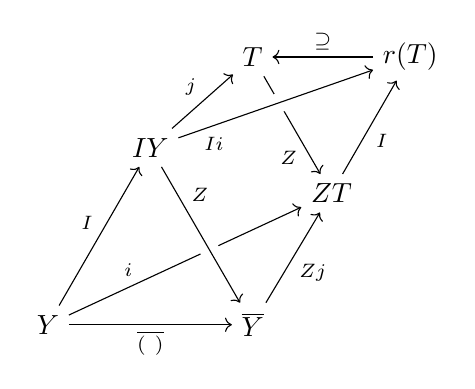
\begin{tikzpicture}[commutative diagrams/every diagram]
%\draw [help lines] (0,0) grid (5,5);
\node (P0) at (0,0) {$Y$} ;
\node (P1) at (1.3*1,1.3*1.73) {$IY$};
\node (P2) at (1.3*2,0) {$\overline{Y}$};

\node (P3) at (2.6,3.4) {$T$} ;
\node (P4) at (4-.4,3-1.73+.4) {$ZT$};
\node (P5) at (5-.4,3+.4) {$r(T)$};


\path[commutative diagrams/.cd, every arrow, every label]

%FGB to B
(P5) edge node[swap] {$\supseteq$} (P3)

% B to GB
(P3) edge node[swap, pos = .7] {$Z$} (P4)

% GB to FGB
(P4) edge node[swap] {$I$} (P5)

% A to GB
(P0) edge node[pos=.3] {$i$} (P4)

% GFA to GB 
(P2) edge node[swap]   {$Zj$} (P4)

% FA to B
(P1) edge node         {$j$} (P3)

% FA to FGB
(P1) edge [-,line width=7pt,draw=white] (P5)
(P1) edge node[swap,pos=.1] {$Ii$} (P5)

% A to FA
(P0) edge node {$I$} (P1)

% FA to GFA
(P1) edge [-,line width=7pt,draw=white] (P2)
(P1) edge node[pos=.3]{$Z$}  (P2)

(P0) edge node[swap] {$\overline{( \  )}$} (P2)
;
\end{tikzpicture}
\end{center}
%%% END FIG 0 %%%%%

\begin{proposition}
The unit of the adjunction is closure, $Z(I(Y)) = \overline{Y}$
\end{proposition}

\begin{proposition}[Hilbert's Nullstellensatz]
The counit of the adjunction is the radical, $r(T) = I(Z(T))$.
\end{proposition}




\end{document}